
\section{Real-Time Data Streaming and Remote Control}
An ESP32-S3 microcontroller serves as the central communication hub between the two-wheeled mobile base, TeraRanger Multiflex ToF sensors, and an external control system. This setup enables real-time data streaming and remote control over Wi-Fi, facilitating remote operation and monitoring. Alternatively, an Arduino Uno R4 WiFi can also be used for similar functionality.

\subsection{System Architecture}  
ESP32-S3 utilizes its SoftAP (Software Access Point) mode to create a dedicated Wi-Fi network, allowing external devices to connect directly without requiring a separate router.
This enables seamless command transmission and telemetry retrieval. The communication architecture includes:

\begin{itemize}
	\item \textbf{TeraRanger Multiflex ToF Sensors}: Connected via UART1 (115200 baud), transmitting real-time distance measurements.
	\item \textbf{Mobile Base}: Communicates via UART2 (9600 baud) using structured command packets for motion control.
	\item \textbf{Wi-Fi Server}: Handles client connections, facilitating bidirectional data exchange. 
\end{itemize}

The ESP32 is configured as following:
\begin{lstlisting}[style=cppstyle2]
// Initialize TerraRanger communication on UART1 (115200 baud rate)
sensorSerial.begin(115200, SERIAL_8N1, 18, 17); // RX = Pin 18, TX = Pin 17
	
// Initialize robot communication on UART2 (9600 baud rate)
robotSerial.begin(9600, SERIAL_8N1, 16, 15);     // RX = Pin 16, TX = Pin 15

// Set up the ESP32 as an Access Point (SoftAP) with SSID and password
WiFi.softAP(SSID, PASSWORD);

// Start the web server to handle client connections
espServer.begin();
\end{lstlisting}


\subsection{Live Data Streaming}
 The system continuously transmits sensor readings for remote monitoring. The implementation includes:

\begin{itemize}
	\item \textbf{Wi-Fi Client Communication:} The ESP32-S3 streams sensor data to a remote server over a TCP socket, ensuring low-latency updates.
	\item \textbf{Telemetry Data Format:} Sensor readings, including ToF and robot state, are formatted and sent in ASCII.  
	\item \textbf{Error Handling:} Ensures stable data transmission by checking connection status before sending.  

	
	\item \textbf{Sensor Data Forwarding}: The ESP32-S3 reads ToF sensor data via UART1 and Robot state data via UART2:
	\begin{lstlisting}[style=cppstyle2]		
void forwardToFData() {
  if (sensorSerial.available()) {
	String tofData = sensorSerial.readStringUntil("\n");
	String data = tofData + "\n";
	sendDataToPC(data);
  }
}
	\end{lstlisting}
	\begin{lstlisting}[style=cppstyle2]		
void forwardRobotData() {
  if (robotSerial.available()) {
	teleData.readUartASCII(robotSerial);
	String data = String(teleData.robotYawDegrees) + "," +
	String(teleData.robotDistanceCm) + "," +
	String(teleData.ultrasonicDistanceCm) + "\n";
	transmitDataToPC(data);
  }
}
	\end{lstlisting}
	\item \textbf{TCP-Based Communication}: The ESP32-S3 establishes a persistent connection with the PC server, periodically sending telemetry updates while ensuring data integrity:
	\begin{lstlisting}[style=cppstyle2]
void transmitDataToPC(const String& data) {
  if (pcClient.connect(SERVER_IP, SERVER_PORT)) {
	pcClient.print(data);
  } else {
	DEBUG_PRINT(DEBUG_COMM, "Failed to connect to PC server!");
  }
  pcClient.stop();  // Close the connection
}
	\end{lstlisting}
\end{itemize}

The Fig.~\ref{fig:live-data-streaming} displays the real-time sensor data received from the robot, visualized in a polar plot.
\begin{figure}[H]
	\centering
	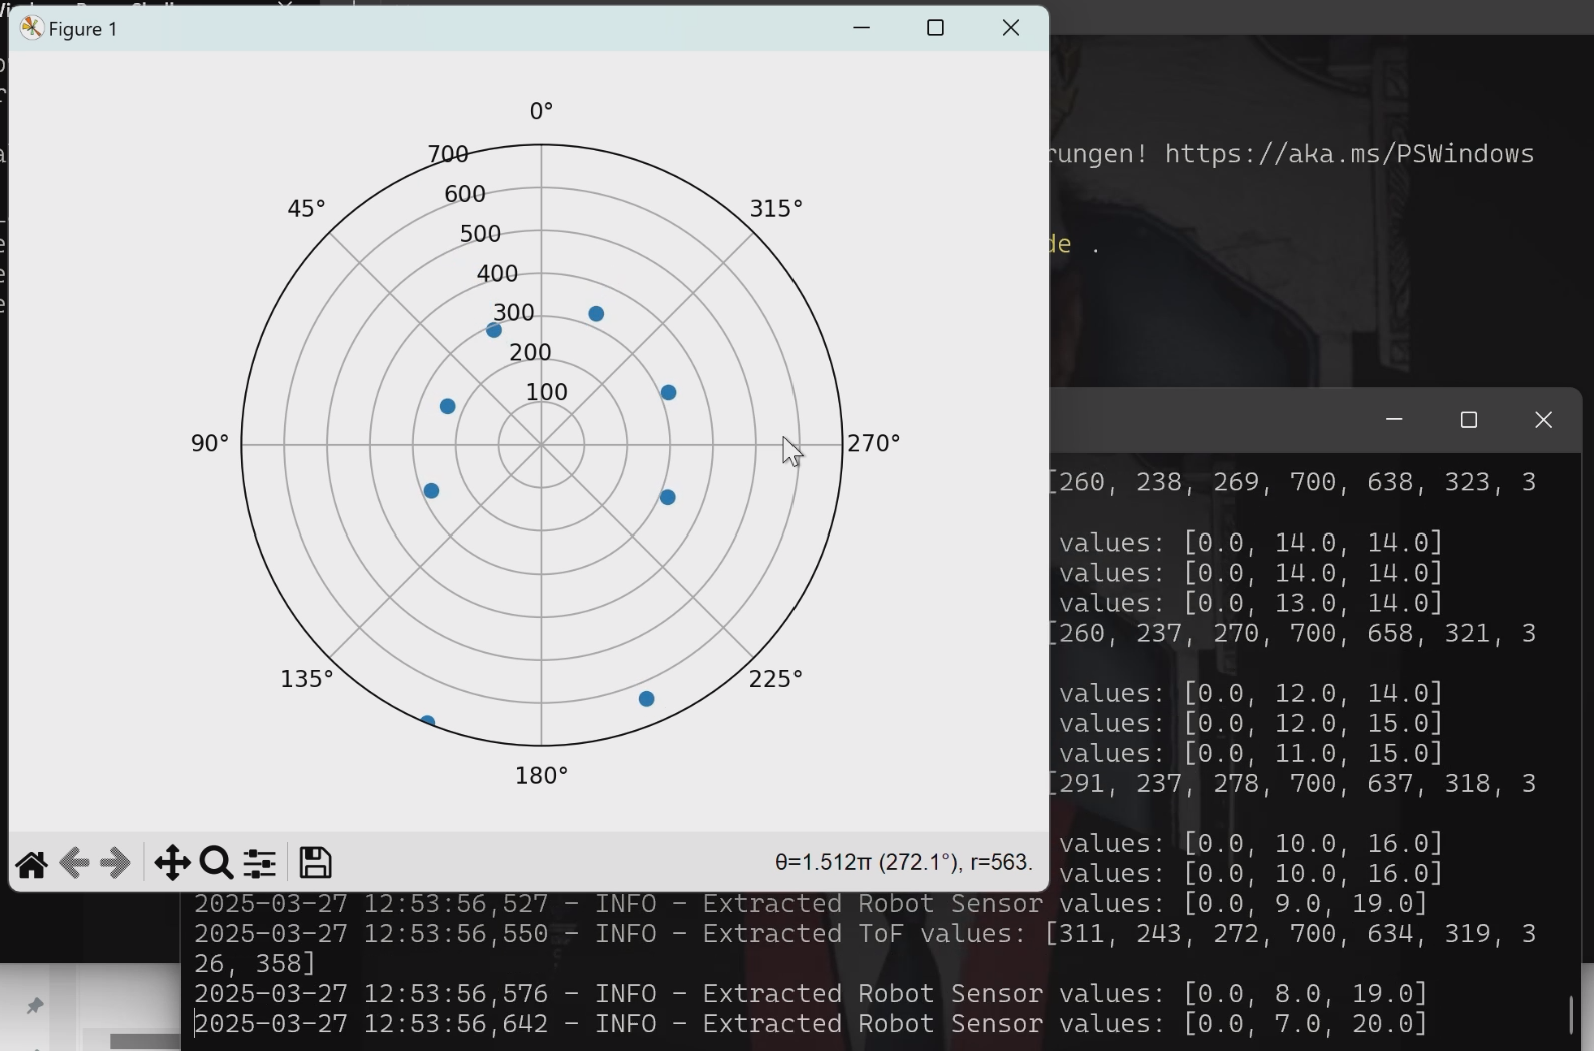
\includegraphics[height=9cm]{assets/LiveDataStreaming.png}
	\caption{Real-time sensor data visualization in a polar plot.}
	\label{fig:live-data-streaming}
\end{figure}


\subsection{Remote Command Processing}External devices can send movement commands to the ESP32-S3, which then interprets and executes them accordingly. The process involves:

\begin{itemize}
	\item \textbf{Command Reception via Wi-Fi Server}: The ESP32-S3 listens for incoming commands over a TCP connection from a remote PC or controller:
\begin{lstlisting}[style=cppstyle2]
WiFiClient client = espServer.available();
if (client) {
	String clientMessage = "";
	while (client.connected() || client.available()) {
		char c = client.read();
		clientMessage += c;
	}
	processCommand(clientMessage);
	client.stop();
}
\end{lstlisting}
	\item \textbf{Command Parsing and Execution}: Received commands are parsed into structured data packets and transmitted to the mobile base via UART2:
\begin{lstlisting}[style=cppstyle2]
int comma1 = command.indexOf(',');
int comma2 = command.indexOf(',', comma1 + 1);
String cmd = command.substring(0, comma1);
int value = command.substring(comma1 + 1, comma2).toInt();
int speed = command.substring(comma2 + 1).toInt();
\end{lstlisting}
	\item \textbf{Supported Commands}: The ESP32-S3 processes commands such as MOVE, ROTATE, and STOP, translating them into appropriate motor control instructions:
\begin{lstlisting}[style=cppstyle2]
if (cmd == "ROTATE") {
	cmdData.command = TumblerCommand::Rotate;
} else if (cmd == "MOVE") {
	cmdData.command = TumblerCommand::Move;
} else if (cmd == "STOP") {
	cmdData.command = TumblerCommand::Stop;
}
cmdData.sendUartASCII(robotSerial);
\end{lstlisting}
	\item \textbf{Client Handling}: Upon receiving a command, the ESP32-S3 acknowledges the request and ensures proper execution before closing the client connection.
\end{itemize}

\section{Final Assembly}
\begin{figure}[H]
	\centering
	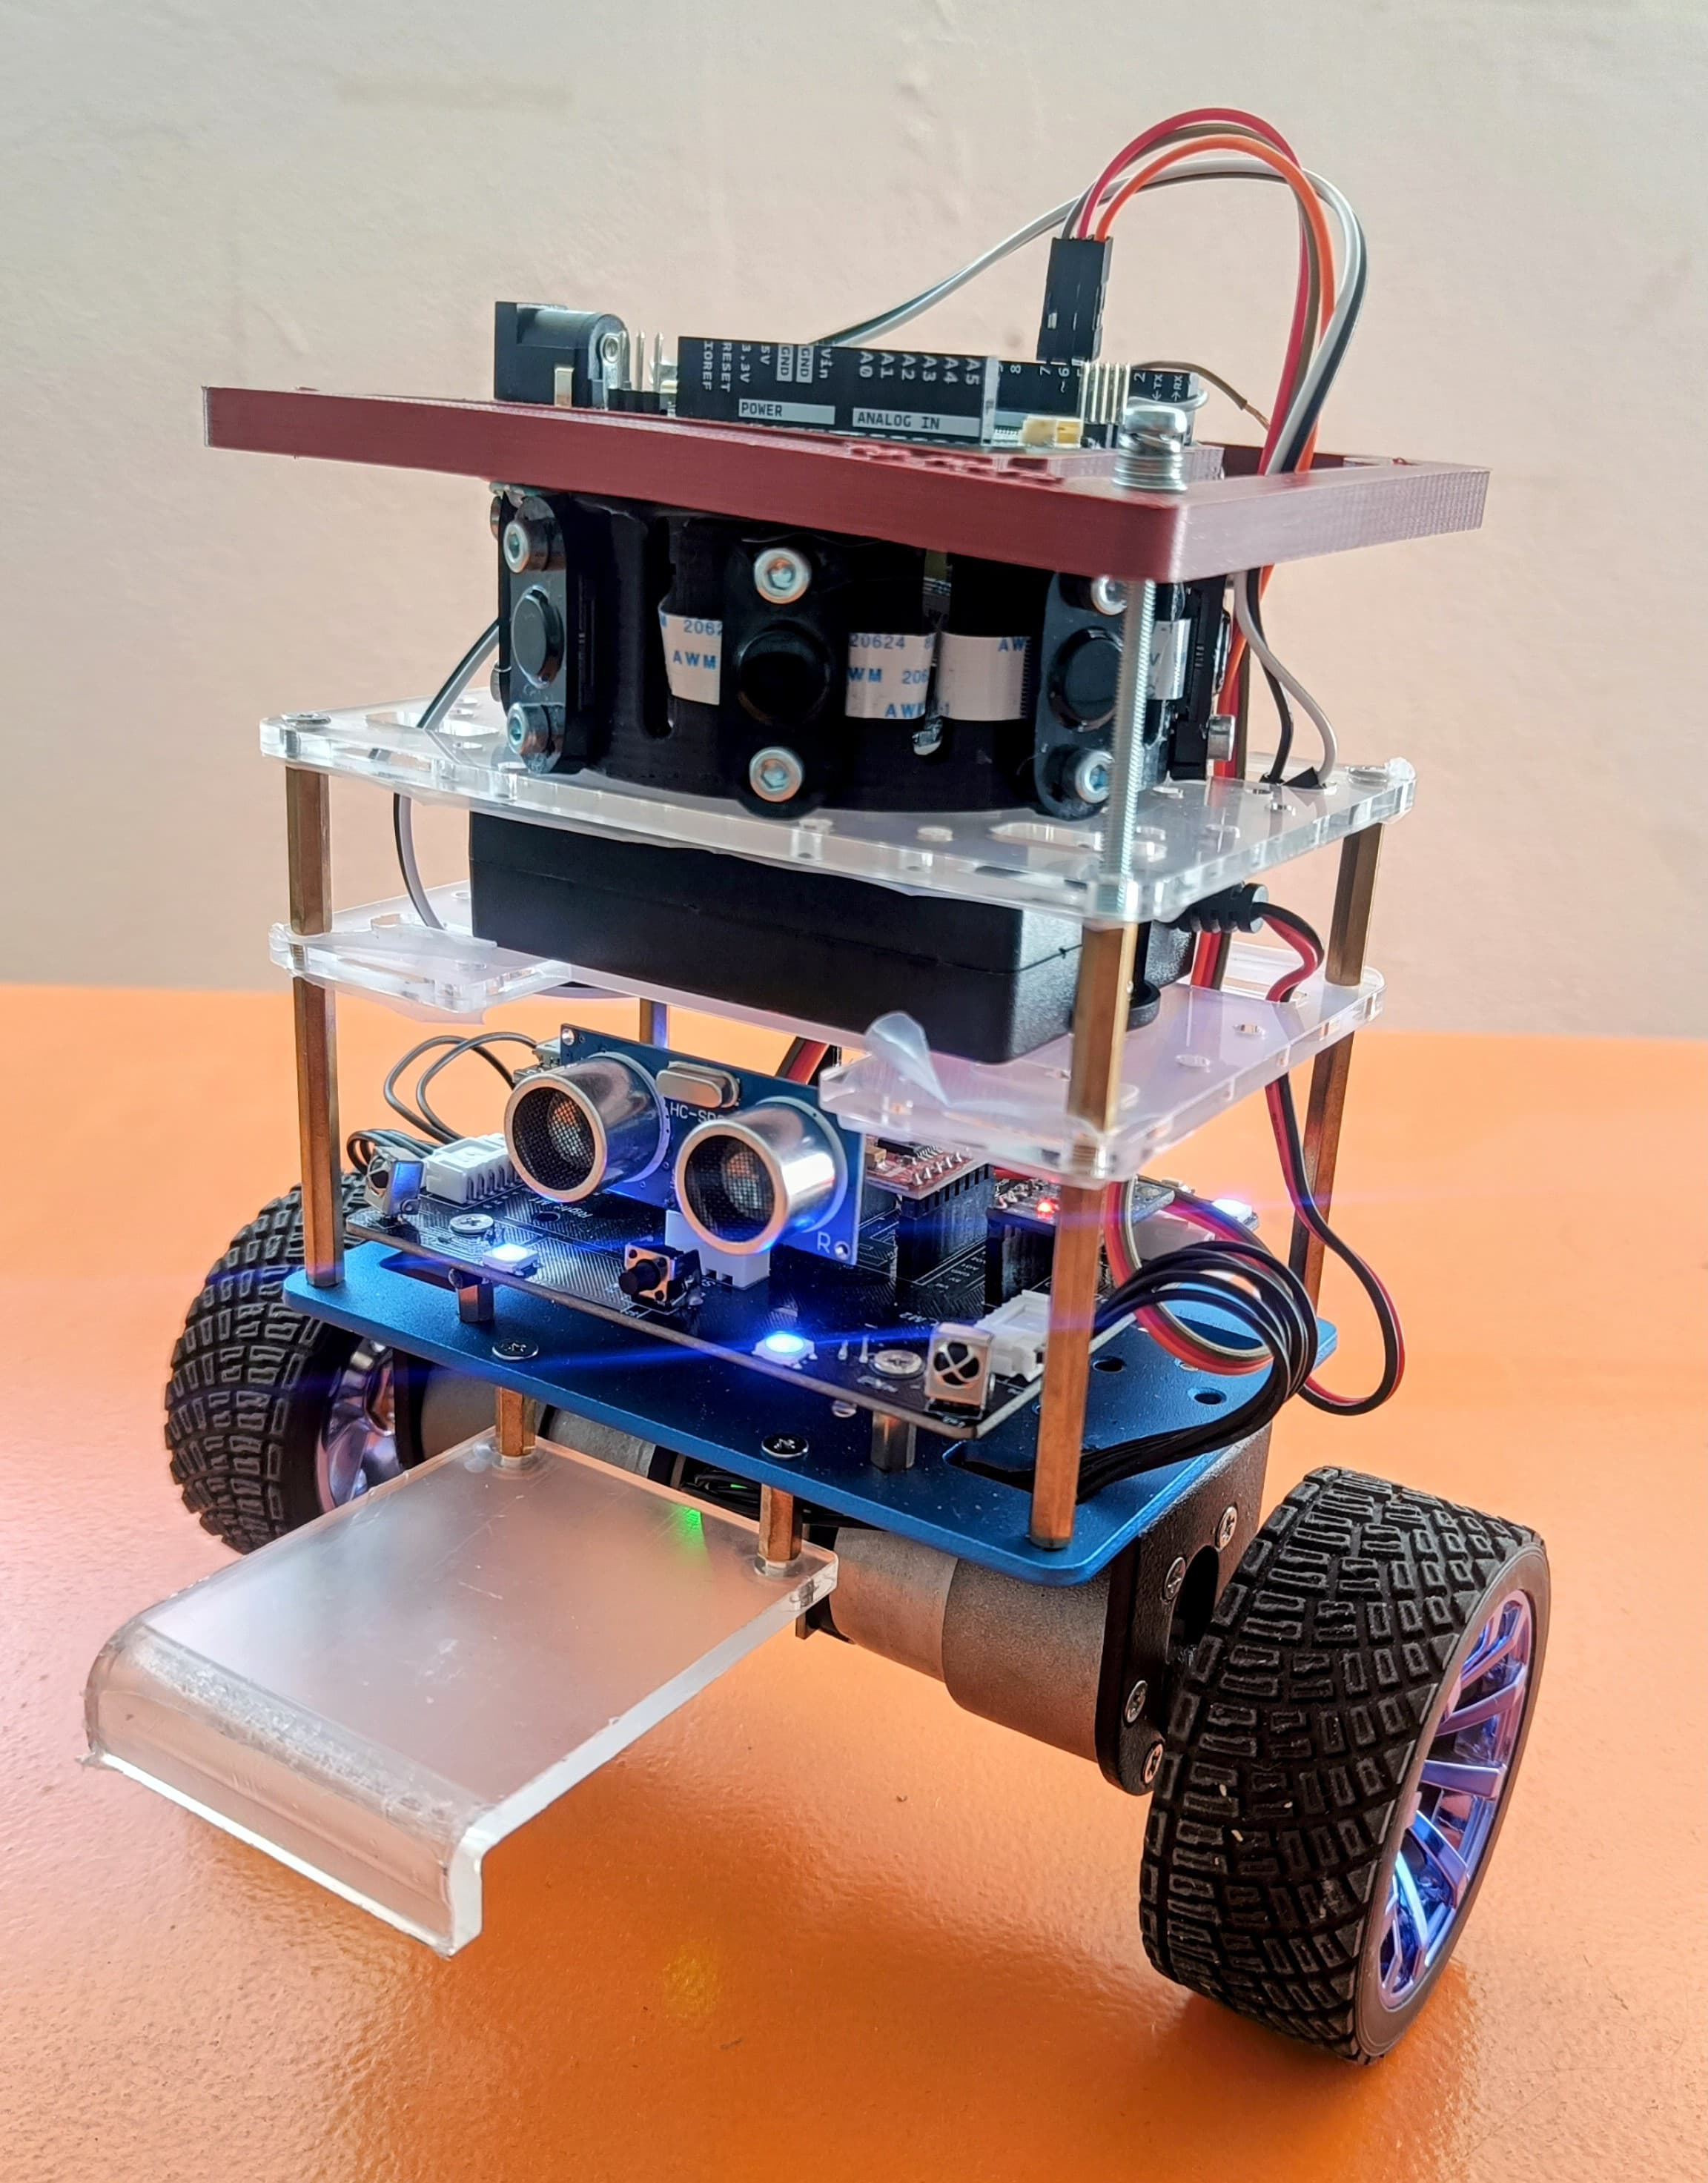
\includegraphics[height=22cm]{assets/RobotFinalAssembly1.jpeg}
	\caption{TeraRanger Multiflex mounted on the mobile base.}
	\label{fig:terraAssembly1}
\end{figure}
